\begin{comment}
\begin{frame}[fragile]
\frametitle{Example: Rohwer data, Ability and PA tests}
\begin{CodeInput}
R> library(candisc)
R> data(Rohwer, package="heplots")
R> cc <- cancor(cbind(SAT, PPVT, Raven) ~ n + s + ns + na + ss, 
+          data=Rohwer, set.names=c("PA", "Ability"))
R> cc
\end{CodeInput}

\begin{CodeOutput}
Canonical correlation analysis of:
         5   PA  variables:  n, s, ns, na, ss 
  with   3   Ability  variables:  SAT, PPVT, Raven 

    CanR  CanRSQ   Eigen percent    cum                          scree
1 0.6703 0.44934 0.81599   77.30  77.30 ******************************
2 0.3837 0.14719 0.17260   16.35  93.65 ******                        
3 0.2506 0.06282 0.06704    6.35 100.00 **                            

Test of H0: The canonical correlations in the 
current row and all that follow are zero

     CanR  WilksL      F df1   df2  p.value
1 0.67033 0.44011 3.8961  15 168.8 0.000006
2 0.38366 0.79923 1.8379   8 124.0 0.076076
3 0.25065 0.93718 1.4078   3  63.0 0.248814
\end{CodeOutput} 
\end{frame}
\end{comment}

\begin{frame}[fragile]
\frametitle{CCA Example: Rohwer data, Ability and PA tests}
\begin{itemize*}
	\item \func{plot} method shows canonical variates for $\mat{X}$ and $\mat{Y}$ on one dimension
	\item Smoother shows possible non-linearity
	\item Point identification highlights unusual observations
\end{itemize*}
\begin{CodeInput}[baselinestretch=0.75]
R> library(candisc)
R> cc <- cancor(cbind(SAT, PPVT, Raven) ~ n + s + ns + na + ss, 
+          data=Rohwer, set.names=c("PA", "Ability"))
R> plot(cc, smooth=TRUE, id.n=3)
R> plot(cc, smooth=TRUE, id.n=3, which=2)
\end{CodeInput}

% two figs side-by-side
  \hfill
  \begin{minipage}[c]{.35\textwidth}
   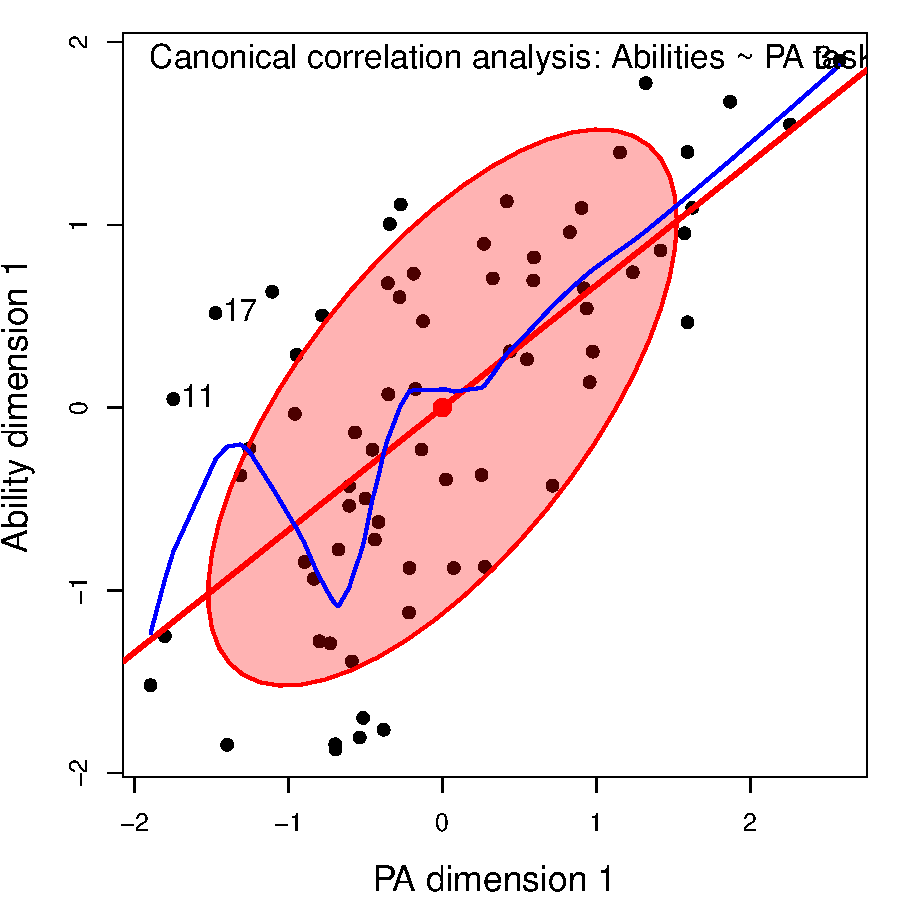
\includegraphics[width=1\linewidth,clip]{figures/rohwer-cancor}
   \end{minipage}%
  \hfill
  \begin{minipage}[c]{.35\textwidth}
   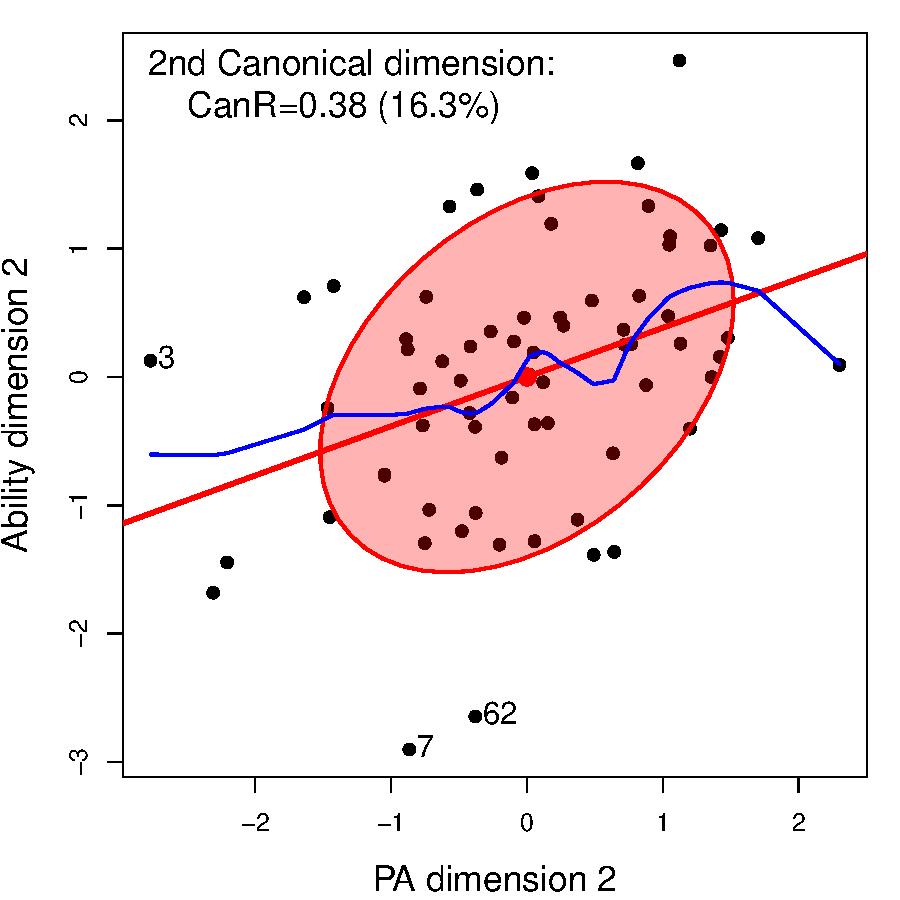
\includegraphics[width=1\linewidth,clip]{figures/rohwer-cancor2}
  \end{minipage}
  \hfill
\end{frame}
